% !TEX root = dissertation_BB.tex
%% spellcheck-language en-US

%  ####
%      #
%   ###
%  #
%  #####

\chapter{Dual Mouse-SPIM}

\graphicspath{{./figures/2_DualMouse/}}

% \section{Challenges in imaging mouse pre-implantation development}
  mammalian development
  chromosome segregation
  cell specification
  symmetry breaking
  signaling pathways
  human infertility
  congenital diseases 

  current mouse-SPIM \cite{strnad_inverted_2016} already is very good for answering many of these questions
  resolution from beads: 
  diSPIM \cite{wu_spatially_2013}
  combine these two
  plus also \cite{balazs_development_2013}

  advantages:
    immersion liquid and culture medium separated
    open-top sample holder allow standard microdrop \textit{in vitro} embryo culture
    row of embryos - high throughput
    dual color imaging
    environmental chamber allows live imaging for 3 days, every 

  follow chromosomes by tracking kinetochores

  from lattice paper: ``because photodamage mechanisms that scale supralinearly with peak intensity have been identified for both visible \cite{donnert_major_2007} and two-photon \cite{ji_high-speed_2008} excitation."


  % ########  ########  ######  ####  ######   ##    ## 
  % ##     ## ##       ##    ##  ##  ##    ##  ###   ## 
  % ##     ## ##       ##        ##  ##        ####  ## 
  % ##     ## ######    ######   ##  ##   #### ## ## ## 
  % ##     ## ##             ##  ##  ##    ##  ##  #### 
  % ##     ## ##       ##    ##  ##  ##    ##  ##   ### 
  % ########  ########  ######  ####  ######   ##    ## 

\section{Microscope design principles}
  In order to address the challenges outlined in the previous section, we propose a new light-sheet microscope design for imaging pre-implantation development at high resolution. The design is guided by the following requirements:
  \begin{enumerate}
    \item subcellular, isotropic resolution
    \item high light collection efficiency
    \item live embryo compatible
  \end{enumerate}

  design principles:
  highest isotropic resolution, highest light collection efficiency possible
  2x0.8 NA water dipping in \SI{90}{\degree} multi-view deconvolve Gaussian fit $\sigma_{xyz}=135$
  2x1.1 NA water dipping in \SI{120}{\degree} multi-view deconvolved Gaussian fit $\sigma_z = 135$, and $\sigma_{xy} = 82.2$
  simulations from PSF generator! put here

  \subsection{Light collection efficiency of an objective}
    Resolution is not the only parameter of concern when designing a new microscope setup. We also have to consider light collection efficiency, since many application, especially live imaging applications require a tight photon budget. This means a single fluorophore can only emit so many times before it undergoes an irreversible chemical reaction, i.e. it bleaches. The more we can collect of these photons, the more information we gain, and altogether the efficiency is higher.

    Photon collection efficiency also defines single molecule localization accuracy, since the signal to noise ratio will depend on the square of the number of collected photons. This is why it's important to also maximize light collection efficiency.

    Let's define light collection efficiency $\eta$ as the ratio of collected photons and all emitted photons:
    \[
    \eta = \frac{N_{collected}}{N_{emitted}}
    \]
    Since we can assume that the direction of photons emitted from a fluorescent molecule are random, the light collection efficiency will correspond to the solid angle subtended by the objective front lens at the focal point. To calculate this, let's consider the unit sphere centered at the focal point, and calculate the surface area of the spherical cap corresponding to the objective acceptance angle $\alpha$ (Fig. \ref{fig:light_effa}). The area of the cap can be expressed as a function of the angle:
    \[
    A_{cap} = 2\pi r^2 (1-\cos \alpha)
    \]
    The surface area of the full sphere is calculated as:
    \[
    A_{sph} = 4 \pi r^2
    \]
    For both equations $r$ is the radius of the sphere. From here, the light collection efficiency can be calculated as:
    \[
    \eta = \frac{N_{collected}}{N_{emitted}} = \frac{A_{cap}}{A_{sph}} = \frac{1-\cos \alpha}{2}
    \]

    Some more calculations: (Fig. \ref{fig:light_effb}).

    \begin{figure}[tpb]
      \centering
    \begin{subfigure}[t]{0.39\textwidth}
      \centering
      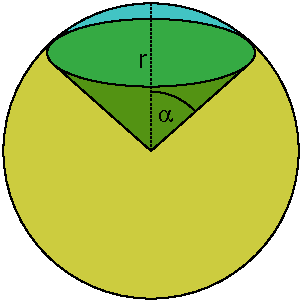
\includegraphics[page=1,width=0.8\textwidth]{efficiency/sphere}
      \caption{\textbf{}}
      \label{fig:light_effa}
    \end{subfigure}
    \begin{subfigure}[t]{0.39\textwidth}
      \centering
      \includegraphics[page=1,width=1\textwidth]{efficiency/light_eff}
      \caption{\textbf{}}
      \label{fig:light_effb}
    \end{subfigure} 
    \bcaption[Light collection efficiency of an objective]{\textbf{(a)} Light collection efficiency is the ratio of photons collected by the objective and all emitted photons. If the fluorophores are emitted randomly in all directions, it will be the surface ratio of the conical section (blue) to the whole sphere. \textbf{(b)} Light collection efficiency ($\eta$) as a function of the numerical aperture (NA)}
    \label{fig:light_eff}
    \end{figure}

  \subsection{Multi-view resolution}
    here a figure with rotating 2 psfs
    \begin{figure}[bt]
      \centering
      \begin{subfigure}[t]{0.45\textwidth}
        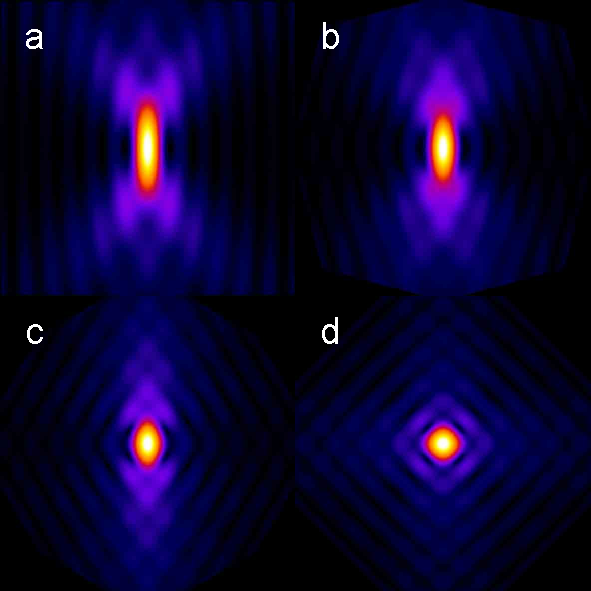
\includegraphics[width=\columnwidth]{simu/psf}
      \end{subfigure}	
      \begin{subfigure}[b]{0.5\textwidth}
      \qquad e
      
        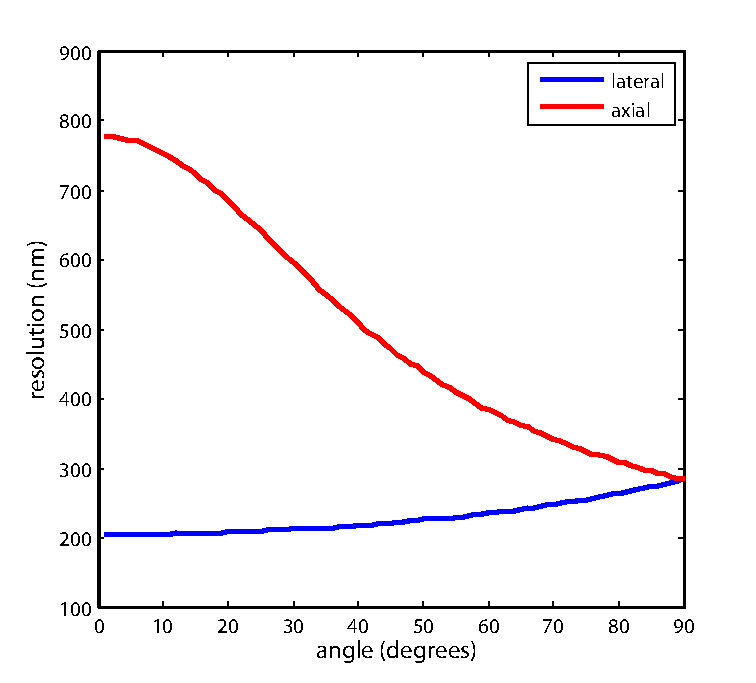
\includegraphics[width=\columnwidth]{simu/resolution}
      \end{subfigure}
      \bcaption[Lateral and axial resolution of a multi-view optical system.]{a) Simulated PSF for a single view. b)--d) Simulated compound PSF of two views aligned in b) 30, c) 60 and d) 90 degrees to each other. e) Axial and lateral resolution of a dual-view setup depending on the rotation angle of the two objectives. Parameters used for calculations: NA=1.1, $\lambda_{ex}=488$nm, $\lambda_{det}=510$nm, $n=1.333$ for water immersion.}
      \label{fig:psf-rot}
    \end{figure}

    \begin{figure}[bt]
      \centering
      \begin{subfigure}{0.49\textwidth}
        \centering
        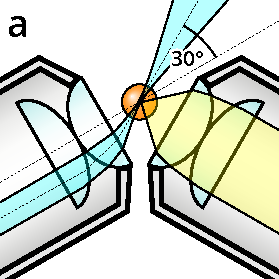
\includegraphics[page=1,width=0.8\textwidth]{objectiveCloseup}
      \end{subfigure}
      \begin{subfigure}{0.49\textwidth}
        \centering
        \includegraphics[page=2,width=0.8\textwidth]{objectiveCloseup}
      \end{subfigure}
      \bcaption[Dual view concept with high NA objectives]{To achieve multi-view detection while maximizing resolution and light collection efficiency, two high NA objectives are placed in \SI{120}{\degree} arrangement. To be able to overlap the light-sheet with the focal plane, the light-sheet is tilted \SI{30}{\degree}. Because of the high NA objectives, this tilt does not effect the illumination quality. The objectives are used in an alternating sequence for illumination and detection.}
      \label{fig:objectiveCloseup}
    \end{figure}

    

    In order to maximize light-collection efficiency and resolution, we opted for a high-NA water dipping objective, the Nikon CFI75 Apo LWD 25x/1.1w model. Two of these arranged in \SI{120}{\degree} allows for twice improved light collection efficiency compared to the 0.8 NA configuration in \SI{90}{\degree} alignment, with further improved lateral resolution along 2 axes (\autoref{fig:psf-rot}). In the next section we will describe the design considerations for illumination and detection optics to achieve optimal sample illumination.

  \subsection{Light-sheet design}
    \label{sec:ls-design}
    To allow for flexibility in the field of view height, even illumination, reduced stripes, and potential for confocal line detection, we opted to use the beam scanning technique to generate a virtual light-sheet. The effective focal length of the Nikon 25x objective, given the \SI{200}{mm} focal length tube lens is
    \begin{equation}
    f_{o} = \frac{f_{tl}}{M} = \frac{200\text{  mm}}{25} = 8 \text{  mm},
    \end{equation}
    and the back aperture diameter is \SI{17.6}{mm}.
    
    To generate the tilted light-sheet as shown on Fig. \ref{fig:objectiveCloseup}, the illumination beam will need to be displaced by
    \begin{equation}
      \delta = f_o \cdot \tan \SI{30}{\degree} = \SI{4.62}{mm}
    \end{equation}
    
    Since the Gaussian beam is not uniform, only a smaller portion of it can be used to maintain even illumination (\autoref{fig:fov}). Because the size of an early mouse embryo is around \SI{80}{\micro m}, we require the length and the height of the light-sheet to be at least \SI{100}{\micro m}.
    

    \subsubsection{The length and thickness of the light-sheet}
    
      As we saw in \autoref{sec:dimensions}, the length of the light-sheet is determined by the Rayleigh-range of the beam in the $zy$ plane. Since $l_{fov}=2\cdot z_{R}=\SI{100}{\micro m}$
      \begin{equation}
        z_{R}=\SI{50}{\micro m}
      \end{equation}
      Since the Rayleigh range and the diameter of the beam waist are coupled, the light-sheet thickness can be calculated after rearranging \autoref{eq:rayleigh}
      \begin{equation}
        2\cdot W_{0} = 2\cdot \sqrt{\frac{z_R \cdot \lambda}{\pi}} = \SI{5.57}{\micro m}
      \end{equation}
      when $\lambda=\SI{488}{nm}$ for GFP excitation. As the beam width for these calculations is defined as $1/e^2$ of the peak intensity, we also calculate the more commonly used FWHM:
      \begin{equation}
        \mathrm{FWHM} = W_0 \cdot \sqrt{2 \ln 2} = \SI{3.28}{\micro m}.
      \end{equation}
      
      From this, the divergence angle of the beam is
      \begin{equation}
        \theta_0 = \frac{\lambda}{\pi W_0,y} = \SI{55.74}{mrad} = \SI{3.196}{\degree}
      \end{equation}
      This means, the numerical aperture needed to produce this light-sheet is:
      \begin{equation}
        \NA_{ls} = n\cdot \sin(\theta _0) = 0.0743
      \end{equation}
      Since $\NA=1.1$, and the diameter of the back aperture is $d=\SI{17.6}{mm}$ and the divergence angle $\theta_0 \ll 1$, using paraxial approximation, the necessary beam width at the back focal plane in the $y$ direction is
      \begin{equation}
        b_y = d \cdot \frac{\NA_{ls}}{\NA} = \SI{1.19}{mm}
      \end{equation}
      Thus, to generate a light-sheet with appropriate length to cover a whole mouse pre-implantation embryo, the laser beam diameter should be $b=\SI{1.19}{mm}$. Larger than this will result in a more focused beam, and a shorter light-sheet, while a smaller diameter beam will have worse optical sectioning capabilities.

    \subsubsection{The height of the light-sheet}
    
    The height can be adjusted by changing the beam scanning amplitude with the galvo mirror. To scan the entire field of view of $h_{fov} \SI{270}{\micro m}$, the scanning angle range at the back focal plane of the objective will need to be $ \theta = \tan^{-1}(h_{fov}/2/f_o) = \pm \SI{0.967}{\degree}$.


      

%  #######  ########  ######## ####  ######   ######  
% ##     ## ##     ##    ##     ##  ##    ## ##    ## 
% ##     ## ##     ##    ##     ##  ##       ##       
% ##     ## ########     ##     ##  ##        ######  
% ##     ## ##           ##     ##  ##             ## 
% ##     ## ##           ##     ##  ##    ## ##    ## 
%  #######  ##           ##    ####  ######   ######  

\section{Optical layout}
  
  Based on the requirements and other considerations layed out in the previous section, the microscope was designed based on three main parts: 1) the core unit, 2) illumination and 3) detection branches. The aim when integrating everything together was to allow for high level of flexibility with robust operation, while keeping efficiency at a high level. After finalizing the concept, the optical layout of the microscope was designed in SolidWorks.

  % \begin{figure}[bth]
  %   \centering
  %   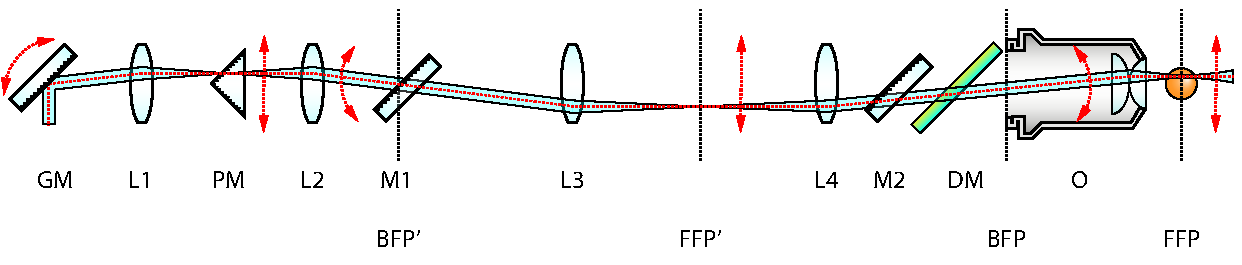
\includegraphics[page=1,width=1\textwidth]{schematicsLinear}
  %   \bcaption[Simplified schematics for illumination]{}
  %   \label{fig:schematicsLinear}
  % \end{figure}


  \subsection{Core unit}
  \label{sec:core}
    \begin{figure}
      \centering
      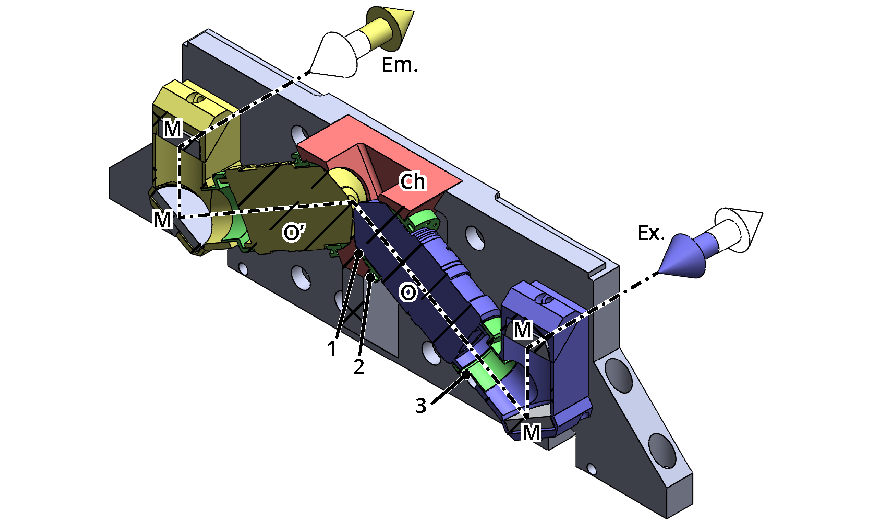
\includegraphics[width=0.8\textwidth]{SW/frontRender.png}
      \bcaption[The core unit of the microscope]{The two objectives (O and O') are mounted on a solid \SI{15}{mm} thick aluminium plate. Fitting on the objectives, a custom chamber (Ch) is holding the immersion medium for imaging. The mirror block with mirrors M3 and M4 directs the light to \SI{65}{mm} optical rails. Excitation (Ex.) and emission (Em.) light paths are indicated by the dash-dot line. Due to the symmetric arrangement, the excitation and illumination paths can be switched around. Objectives are secured with rings 1--3 (green, see main text for details).}
      \label{fig:Core}
    \end{figure}

    As the most important part of the microscope is actually the sample, the design is based around a core consisting of the imaging chamber and the objectives (\autoref{fig:Core}). Also part of the core are two mirror blocks placed at the back of the objectives, and three custom designed rings to hold the objectives in place. The objectives are pointing slightly up, closing a \SI{60}{\degree} angle with the horizontal plane, and \SI{120}{\degree} angle with each other. 

    \subsubsection{Chamber}
    The chamber serves two purposes: it holds the immersion liquid necessary for imaging, and it also keeps the objectives in the \SI{120}{\degree} position. The objectives are held by their necks as opposed to the standard mounting method from the back by the threads. The advantage of this is that any axial movements due to thermal expansion are greatly reduced, thus the focal plane position is more stable even when changing the imaging conditions.

    The chamber is machined form a high performance plastic, poly(ether-ether-ketone) (PEEK). This material has many beneficial properties: it is food safe, and chemically extremely inert, resisting to most solvents used in a biology laboratory. It can also be autoclaved. Compared to other plastics its mechanical properties are also superior. It has high tensile and compressive strength, comparable to aluminium, low thermal expansion and low thermal conductivity. This can be beneficial when implementing temperature control, as thermal loss is reduced.

    The objectives are kept in place by two custom designed rings (\autoref{fig:Core} 1, 2). The first ring has a cross sectional shape of a wedge, and sits tightly against both the objective and the wall of the chamber. The second ring can freely slide on the objective, and has threads matching the chamber. When turned in, the threaded ring pushes the wedge ring further in, which in turn presses against the objective and the chamber wall uniformly, thus preventing the objective from moving, and sealing the chamber at the same time. As the wedge ring is made from a soft plastic (delrin), it will press evenly against the objective preventing any damage. Because of the conical shape of the ring, it will also automatically center the objective, ensuring correct positioning.

    To relieve any rotational stresses from the objective, the back of the objective is also supported  by the mirror block, this is not fixed, however. A third ring, made of PEEK is screwed on the thread of the objective, and slides in the opening of the mirror block. This reduces the torque on the objectives, while still allowing for some movements that might occur due to thermal expansion.

    \subsubsection{Mirror blocks}
    \label{sec:mirrors}
    Apart from supporting the objectives from te back, the mirror blocks are housing two broadband dielectric mirrors (Thorlabs, BBE1-E03 and OptoSigma, TFMS-30C05-4/11) to direct the light in and out from the objectives on a standard \SI{65}{mm} height, compatible with the Owis SYS65 rail system. The combination of two mirrors have two benefits compared to using just one. With a single mirror directly reflecting the light to the back, the entire assembly would need to be much higher to reach the desired \SI{65}{mm} height. This could result in stability problems. Furthermore, due to the \SI{60}{\degree} rotation angle of the objective, the image of the objective would also be rotated if using only a single mirror. With two mirrors the reflection planes can be kept orthogonal to the optical table, which will result in a straight image after the mirror block. This is not only beneficial when recording the images, but also when aligning the illumination arm. With the use of two mirrors, a convenient vertical scanning is required to produce the light-sheet; with a single mirror, the scanning direction would need to be rotated by \SI{60}{\degree}.


  \subsection{Illumination}
    \begin{figure}[bt!]
      \centering
      \begin{subfigure}{\textwidth}
        \centering
        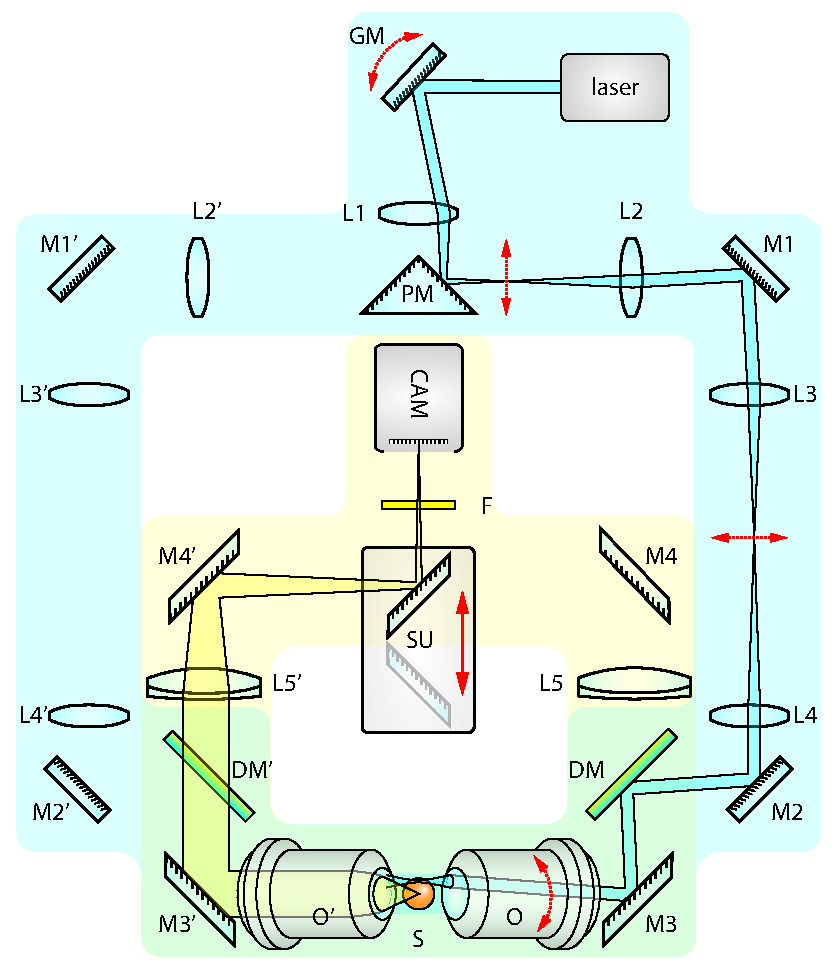
\includegraphics[page=1,width=0.9\textwidth]{fullSchematics}
      \end{subfigure}
      \begin{subfigure}{\textwidth}
        \centering
        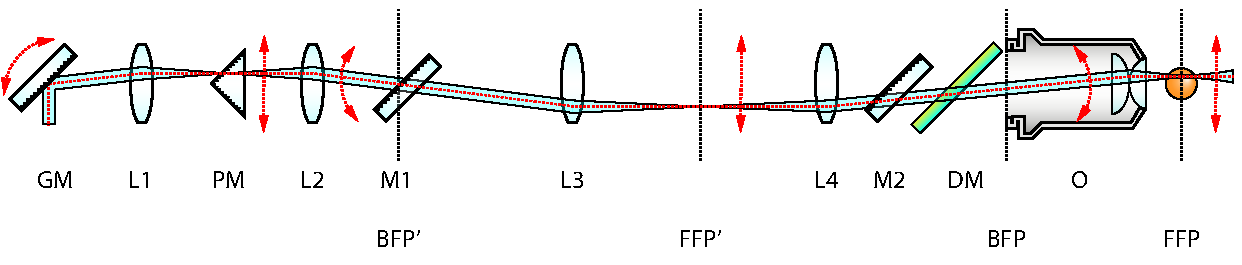
\includegraphics[page=1,width=1\textwidth]{schematicsLinear}
      \end{subfigure}
      
      \bcaption[Dual Mouse SPIM optical layout]{The microscope consists of two main parts, the illumination branches (blue) and detection branches (yellow). For both illumination and detection there are two identical paths implemented. Illumination direction can be changed by applying a different offset to the galvo mirror, which in turn will direct the beam to the opposite face of the prism mirror. L1 and L2 will then image the galvo on M1. Using L3 as a scan lens, and L4 as a tube lens, the scanned beam is coupled to the objective path by quad band dichroic mirror (DM)
      CAM -- camera, DM -- dichroic mirror, F -- filter wheel, L -- lens, M -- mirror, O -- objective, PM -- prism mirror, S -- sample}
      \label{fig:fullSchematics}
    \end{figure}

    The illumination arm of the microscope directs and shapes the laser beam to generate the proper light-sheet dimension at the sample. As was calculated in \autoref{sec:ls-design}, a beam diameter of \SI{1.2}{mm} is ideal for this setup.

    The illumination arm has 3 main roles:
    \begin{enumerate}
      \item expands the laser beam to the calculated \SI{1.2}{mm} size.
      \item images the galvo scanner to the back focal plane of the objective
      \item switches the laser light between the two objectives during imaging
    \end{enumerate}

    To achieve the desired beam diameter, a 1:2 beam expander (Sill Optics, 112751) is used in the reversed direction. As the output of the laser fiber produces a \SI{3}{mm} diameter beam, this will reduce it to \SI{1.5}{mm}. As this is already the required beam diameter, the lenses further in the illumination path will not introduce any magnification.
    
    % \subsubsection{Beam splitter unit}
    \label{sec:splitter}

    Switching between the two illumination arms is performed by a custom designed beam splitter unit (\autoref{fig:splitter}). Instead of utilizing a 50/50 beam splitter cube and mechanical shutters, we exploit the fact that a galvo scanner is needed to generate the light-sheet. As this galvo scanner (Cambridge Technology, 6210B) has a relatively large movement range ($\pm \SI{20}{\degree}$) it is also suitable for diverting the beam from one illumination arm to the other.

    \begin{figure}[h]
      \centering
      \includegraphics[width=0.8\textwidth]{SW/splitterFigure}
      \bcaption[Illumination branch splitting unit]{To divert the beam to either side, a right angle prism mirror is used in conjunction with a galvanometric scanning mirror. L1 acts as a scan lens, thus the beam is translated on mirror M. Depending on the galvo angle, the beam will be reflected either to the left (\textbf{a}) or to the right (\textbf{b}). L2 and L2' act as relay lenses, and will image the galvo movement to intermediate planes.}
      \label{fig:splitter}
    \end{figure}

    Switching illumination side is done the following way. As the galvo is positioned at the focus of the first lens (L1, $f_1 = \SI{75}{mm}$, Edmunds Optics, \#47-639), the rotational movement will result in a linear scanning movement on mirror M and the prism mirror PM (Thorlabs, MRAK25-E02). Depending on the lateral position of the beam, it will hit either the left or the right leg of the prism, and will be reflected to either direction. As the galvo mirror can be precisely controlled through our custom software, we can set and save the position when the beam is centered on the left lens L2 ($f_2 = \SI{75}{mm}$, Edmunds Optics, \#47-639) (\autoref{fig:splitter}a) and the position when the beam is centered on the right lens L2' (\autoref{fig:splitter}b). Lenses L1 and L2(L2') form a 4f system, and are imaging the galvo scanner on mirror M1(M1') (\autoref{fig:fullSchematics}). This way we can use the same galvo to generate the light-sheet for both directions, depending on the initial offset position. This not only has the advantage of being able to electronically switch the illumination arms, but only requires a single galvo scanner instead of one for each arm.
    
    Due to the arrangement of the bottom mirror and the prism mirror, the scanning direction will be rotated by \SI{90}{\degree}. This will result in a vertical scanning plane, which is exactly what we need to generate the light-sheet on the sample (see \autoref{sec:mirrors}).

    % \subsubsection{the rest of illumination}
    Further following the illumination path, two achromatic lenses L3 and L4 ($f_3 = f_4 = \SI{200}{mm}$), in a 4f configuration relay the scanning axis to the back focal plane (BFP) of the objective. To couple in the laser with the imaging path, a quad-band dichroic mirror (DM, Semrock, Di03-R405/488/561/635-t3-25x36) is used, matching the wavelengths of the laser combiner.

  \subsection{Detection}
    As the emitted light exits the objective and the mirror block, it is decoupled from the illumination path by the dichroic mirror. The light is then focused by a \SI{400}{mm} achromatic lens (L5, Edmunds Optics, \#49-281) onto the camera sensor (Andor Zyla 4.2 sCMOS). Just before the camera, a motorized filter wheel (F, LEP 96A361) is placed to filter out any unwanted wavelength from the emission light. Although this is not in the infinity space, due to the very small angles after the \SI{400}{mm} tube lens, the maximum axial focal shift is $\sim \SI{50}{nm}$ only, which is negligible compared to the axial resolution of $\sim \SI{1.1}{\micro m}$.

    Similarly to the common galvo in the illumination path, the two detection arms share the same camera. Although two cameras could also be used, due to the operating principle of the microscope, the two objective are not used for imaging at the same time. This means a single camera is capable of acquiring all the images, however, the two distinct detection arms need to be merged to be able to use a single camera.
    
    Our solution to this problem is a custom designed view switching unit comprised of two broadband dielectric elliptical mirrors (Thorlabs,BBE1-E03) ) facing opposite directions, mounted on a high precision linear rail (OptoSigma, IPWS-F3090). Depending on the rail position, either the left (\autoref{fig:dualMirror}a) or the right (\autoref{fig:dualMirror}b) detection path will be reflected up, towards the camera. 

    Moving the switcher unit is performed by a small, \SI{10}{mm} diameter pneumatic cylinder (Airtac, HM-10-040) that is actuated by an electronically switchable 5/2 way solenoid valve (Airtac, M-20-510-HN). This solution offers a very fast switching between views, up to \SI{5}{Hz}, depending on the pressure, and it is extremely simple to control, as only a digital signal is necessary to switch the valve. 

      \label{sec:dualMirror}
      \begin{figure}[tb]
        \centering
        \includegraphics[width=0.8\textwidth]{SW/dualMirrorFigure}
        \bcaption[Detection branch switching unit]{To be able to image both views on the same camera, a moveable mirror unit is introduced. Depending on the imaging direction, the mirror block is either moved backward (\textbf{a}) or forward (\textbf{b}) to reflect the light up to the camera. Since the movement is parallel to the mirrors' surface, the image position on the sensor is not dependent on the exact position of the mirrors.}
        \label{fig:dualMirror}
      \end{figure}
        
      


  %    ###    ##       ####  ######   ##    ## 
  %   ## ##   ##        ##  ##    ##  ###   ## 
  %  ##   ##  ##        ##  ##        ####  ## 
  % ##     ## ##        ##  ##   #### ## ## ## 
  % ######### ##        ##  ##    ##  ##  #### 
  % ##     ## ##        ##  ##    ##  ##   ### 
  % ##     ## ######## ####  ######   ##    ## 
\section{Optical alignment}
  Precise alignment of the illumination and detection paths are crucial for high quality imaging, and has a pronounced  importance for high magnification and high resolution optical systems. The DualMouse SPIM contains two illumination and detection paths 
  Due to the symmetrical setup of the microscope, we will only describe the alignment of one side, as the same procedure is also applicable to the other side.

  \subsection{Alignment of illumination branches}

    The two illumination branches start with a common light source, a single mode fiber coupled to laser combiner, and they also share a galvanometric mirror that performs the beam scanning to generate the virtual light-sheet. Likewise shared is a scan lens focusing on the galvo mirror (GM), and the illumination splitter unit (PM, see Section \ref{sec:splitter}).

    Alignment for the illumination arms are done in three steps. First the laser beam is aligned on the first rail that holds the galvo, lens L1, and the splitter unit PM. This is performed by two kinematic mirrors placed between the fiber output and the galvo mirror (not shown on figure). Using these two mirrors it's possible to freely align the beam along all 4 degrees of freedom: translation in two orthogonal directions, and rotation around two orthogonal axes. Beam alignment on the rail is tested by two irises at the two ends of the rail, if the beam passes through both of them we consider it centered and straight on the optical axis.

    After the beam is aligned on the first rail, lens L1 and the splitter unit PM are placed in the measured positions to image the galvo mirror on mirror M1 using lenses L1 and L2. Correct positioning of the splitter unit along the rail is crucial, since this will affect the lateral position and tilt of the beam exiting the unit. To some extent, this can also be compensated by adjusting the two mirrors before the galvo mirror, but is avoided if possible as this will also displace the beam from the center of the galvo mirror.

    After rough alignment of the illumination arms, when the laser is already coupled in the objective, the fine adjustments are performed based on the image of the beam through the other objective. The beam is visualized by filling the chamber with a 0.1\% methylene blue solution. As this solution is fluorescent, and can be excited in a very large range, it is well suited to visualize the beam during adjustment.

    \subsubsection{Adjusting beam position}
      Beam position can be adjusted by either translating the beam in a conjugated image plane (I'), or by rotating the beam in a conjugated back focal plane (BFP'). The setup was designed in a way, that BFP' coincides with mirror M1. This mirror is mounted in a gimbal mirror mount, allowing to rotate the mirror exactly around its center, which avoids unwanted translational movements, and results in pure rotation of the beam. Lens L3 is positioned exactly 1 focal length from the mirror, thus acting as a scan lens, and transforming the rotational movements to translation. This translation is further imaged and demagnified by the tube lens L4 and the objective O onto the sample.


    \paragraph{Adjusting beam tilt}
      Beam tilt can be adjusted by either rotating the beam in an intermediate image plane (I'), or translating it at the back focal plane (BFP). As mirror M2 is relatively far from the back focal plane, adjusting this will mostly result in translation that will rotate the beam. This movement, however will also introduce translations, and has to be compensated by adjusting mirror M1. The light-sheet, however needs to be tilted by \SI{30}{\degree} to coincide with the focal plane of the other objective, and this degree of adjustment is not possible with M2. In order to allow for a pure rotation of the light-sheet, we mounted the dichroic mirrors on a linear stage (OptoSigma, TSDH-251C). By translating the dichroic mirror, the illumination laser beam gets translated at the back focal plane, which will result in a pure rotational movement at the sample. Rough alignment of the light-sheet is performed by adjusting the dichroic position while inspecting the light-sheet through a glass window in the chamber. Precise alignment is then done based on the image of the beam visualized in a fluorescent medium.


    \paragraph{Adjusting beam axial position.}


    \paragraph{Adjusting scanning plane angle.}
      After the beam is properly aligned, i.e. it is in focus, and in the center of filed of view, it is still necessary to check if the scanning direction is parallel to the imaging plane. It is possible that the beam is in focus in the center position, but when moved up or down it drifts out of focus due to a tilted scanning angle. This tilt can be compensated by mirror M1, that is placed at the conjugated back focal plane BFP'. Between lenses L3 and L4 a magnified version of the light-sheet will be visible, and the tilt can be checked by placing an alignment target in the optical path while scanning the beam. By tilting mirror M1 up or down, the scanning pattern not only moves up or down, but is also rotated if the mirror surface is not exactly vertical. Since M1 and GM are in conjugated planes, the tilt and offset can be performed independently. The tilt is first fixed by M1 while inspecting the target, and the beam is re-centered by changing the offset on the galvo mirror. Moving the galvo mirror will not introduce tilt, since in this case rotation axis is perpendicular to the reflection plane.




  \subsection{Alignment of detection branches}
    Since the detection path is equivalent to a wide-field detection scheme, its alignment is much simpler than that of the illumination branches. The only difference is the detection branch merging unit (see \autoref{sec:dualMirror}.) that features two moving mirrors. This, however doesn't effect the alignment procedure, since the movement direction is parallel to both mirror's surface, meaning that the exact position of the mirrors will not affect the image quality, as long as the mirrors are not clipping the image itself. Stability test were performed to confirm the consistent switching performance of the mirror unit before the final alignment took place (see Sec. \ref{sec:mirrorStability}).

    % TODO: complete paragraph
    The final alignment procedure 

    \paragraph{Positioning the tube lens.}
      The position of the tube lens determines the focal plane the is being imaged on the camera sensor. Ideally, the tube lens' distance from the camera sensor is exactly the tube lens focal length, which will ensure the best imaging performance. If the tube lens distance is not correct, the focal plane will be slightly shifted in the axial direction. Although small shifts will not necessarily have detrimental effect on the image quality, because the light sheet can also be shifted accordingly. Because of the shifted focal and image planes, however, the magnification of the system will be affected, and will change depending on the amount of defocus. For this reason we aim for positioning the tube lens as close to the theoretical position as possible.

      Our tube lens is a compound, achromatic lens with a center thickness of \SI{12.5}{mm}, and edge thickness of \SI{11.3}{mm}. Its effective focal length is \SI{400}{mm} which will produce a 50x magnified image. Back focal length is \SI{394.33}{mm} which we measured form the camera chip, and the lens was positioned at this theoretically optimal position.

    \paragraph{Adjusting correction collar.}
      The Nikon 25x objectives used for this setup have a built in correction ring that can be used to correct spherical aberrations resulting from refractive index differences when imaging samples behind a coverslip. This can be also effectively used to correct for any spherical aberrations occurring from imaging through the FEP foil. Although these aberrations are expected to be extremely low, due to the relatively thin, \SI{50}{\micro m} foil thickness, and the close matching of refractive index ($n_{FEP} = 1.344$, $n_{H_2O}=1.333$), for optimal, aberration free image quality it can't be neglected.

      The correction collars are adjusted by inspecting a gel suspended fluorescent bead specimen with the microscope, where the beads can act as a reporter of the point spread function of the microscope. The alignment can be performed ``live" by inspecting the bead image quality for any aberrations. By gradually changing the correction collar, the ring are minimized on out of focus beads, and the peak intensity is maximized for in focus beads. By moving the correction ring, the focal plane is also slightly shifted, which has to be compensated by shifting the light-sheet correspondingly to coincide with the correct imaging plane.

    \paragraph{Adjusting field of view.}
      To allow for proper sampling of the image, we use 50x magnification, which, combined with the \SI{6.5}{\micro m} pixel pitch of our sCMOS camera will result in a \SI{0.13}{\micro m} pixel size. The full field of view with this magnification is $2048 \times 0.13 = \SI{266.24}{\micro m}$. The full field of view the objective provide, are larger than this, at \SI{800}{\micro m}. To ensure the best image quality, we align the center of the objective field of view on the camera sensor, since this region has the best optical properties in term of numerical aperture, aberration correction and field flatness.

      Field of view alignment can be performed using mirror M4 just before the detection merging unit. To identify the center region of the field of view, diffuse white light is used to illuminate the entire sample chamber, and is imaged on the camera. Then, mirror M4 is adjusted until the top edge of the field of view becomes visible, \textit{i.e.} where the illumination from the chamber is clipped. This will have a circular shape. Then, adjusting the mirror in the orthogonal direction, the left-right position of the field of view can be adjusted, by centering the visible arc on the camera sensor.

      After the horizontal direction is centered, vertical centering is performed. This, however can't be centered the same way as the horizontal direction, since for that we would have to misalign the already aligned horizontal position. To determine the center, we move the field of view from the topmost position to the bottom. During this process the number of  turns of the adjustment screw is counted (this can be done accurately by using a hex key). After reaching the far end of the field of view, the mirror movement is reversed, and the screw is turned halfway to reach the middle.







\section{Control unit}

  Apart from the optics design, automation hardware and software is also a custom design. To be able to conduct high speed experiments and time-lapse recordings, a high level of automation, hardware and software integration is necessary. Our system comprises of two main components: a National Instruments embedded system (cRIO 9068), and a high performance workstation.

  \subsection{Hardware}
    Various components need to be properly synchronized to operate the microscope. Illumination is performed with a multi-line laser combiner, light-sheet is generated by a galvo scanner. To discriminate fluorescent light from th excitation light, a motorized filter wheel is used with appropriate long pass and band pass filters (see Appendix \ref{sec:BOM}).
    For more details, see Appendix \autoref{sec:BOM}.

    The different devices require different signals to control them. We can split them into three main categories:

    \begin{center}
      \begin{tabular}{lll}      
        \textbf{digital input} & \textbf{analog input}   & \textbf{serial communication} \\ \hline
        camera exposure    & galvo position & filter wheel         \\
        laser on/off (\texttimes 3) & laser intensity (\texttimes 3) & stages (\texttimes 2)
      \end{tabular}
    \end{center}

    All devices are connected to the NI cRIO 9068 embedded system, either to the built in RS232 serial port, or to the digital and analog outputs of the FPGA card.
  
  \subsection{Software}

    \begin{figure}
      \centering
      \includegraphics[width = 0.6\textwidth]{fpgaTraces}
      \bcaption[Digital and analog control signals]{Example traces for recording a single plane with \SI{50}{ms} exposure time and \SI{12}{ms} delay. During the exposure of the camera the galvo has 3 sections: acceleration (acc.), linear, and deceleration (dec.). The laser line is synchronized with the galvo linear section to ensure even illumination. }
      \label{fig:traces}
    \end{figure}


% ########  ########  ######  ##     ## ##       ########  ######  
% ##     ## ##       ##    ## ##     ## ##          ##    ##    ## 
% ##     ## ##       ##       ##     ## ##          ##    ##       
% ########  ######    ######  ##     ## ##          ##     ######  
% ##   ##   ##             ## ##     ## ##          ##          ## 
% ##    ##  ##       ##    ## ##     ## ##          ##    ##    ## 
% ##     ## ########  ######   #######  ########    ##     ######  
\section{Results}
  \begin{figure}[htb]
    \begin{subfigure}[t]{0.5\textwidth}
      \centering
      \includegraphics[width=\textwidth]{front_solidworks_overlay}
      \caption{Rendering of SolidWorks design.}
    \end{subfigure}
    \begin{subfigure}[t]{0.5\textwidth}
      \centering
      \includegraphics[width=\textwidth]{front_photo_overlay}
      \caption{Photo of constructed microscope.}
    \end{subfigure}
    \bcaption[Front view of the Dual Mouse-SPIM]{}
    \label{fig:frontView}
  \end{figure}

  Resolution for Lattice light-sheet \cite{chen_lattice_2014}: \SI{230}{nm} in x and \SI{370}{nm} in z
  \cite{chhetri_whole-animal_2015}

  After the design phase, all custom parts were manufactured the the EMBL workshop, and microscope was assembled on a NewPort X by X optical table (Fig. \ref{fig:frontView}).

  \subsection{Characterizing illumination profile}
    Since a Gaussian beam is used for illumination, it's intensity profile is dependent on the axial position (Eq. \ref{eq:gaussian}). Although the total intensity at any cross section of the beam is constant, because of the divergent properties, the peak intensity varies. To assess any non-uniformities in the illumination pattern, we measured the illumination beam intensity for each view.

    To visualize the beam, the chamber was filled with a fluorescent solution (methylene blue solution in distilled water). In order to increase the signal to noise ratio of these images, a long exposure time of \SI{200}{ms} were used, and 500 images of each beam was averaged (Fig. \ref{fig:beamProfiles}). The measure Rayleigh range of the left and right beams respectively: "\SI{666}{\micro m}" ans "\SI{666}{\micro m}". The width of the beam, \textit{i.e.} the thickness of the light-sheet are "\SI{666}{\micro m}" and "\SI{666}{\micro m}" for the left and right beams respectively (\autoref{fig:beamProfiles}).

    \begin{figure}[htb]
      \centering
      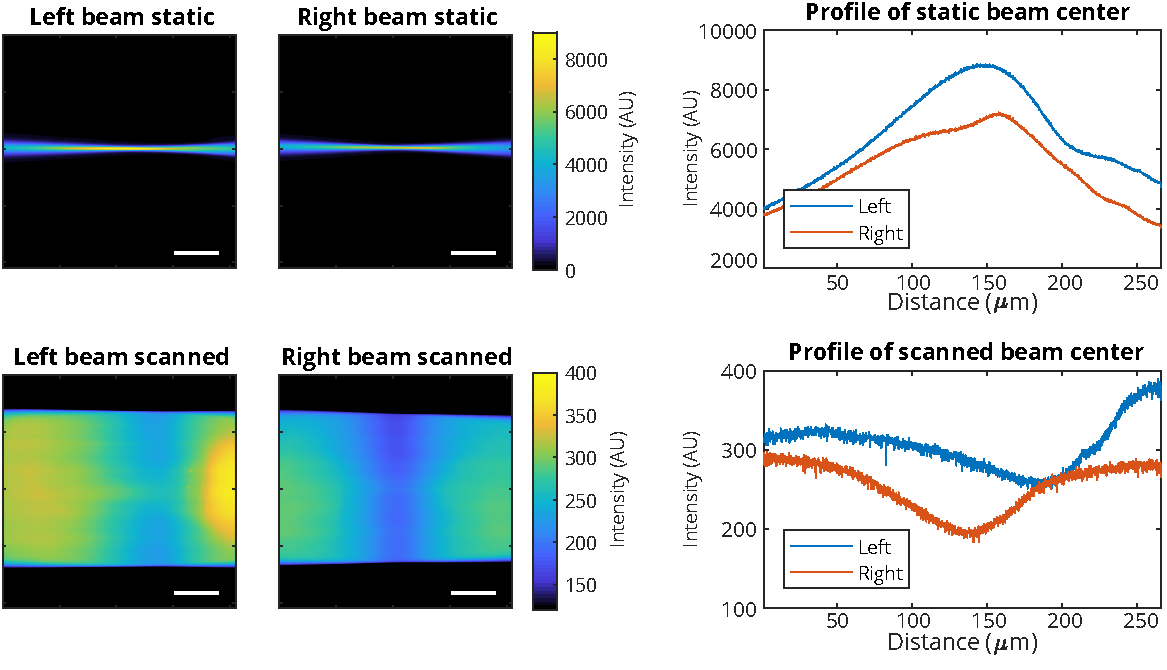
\includegraphics[width=\textwidth]{beamProfile488.pdf}
      \bcaption[Illumination beam profile]{Average of 50 stationary beam images for both left and right objectives (top left). Beam intensity profile along the center of each beam is plotted (top right). To simulate scanned beam illumination intensity, each beam image was averaged along the vertical axis (bottom left). Intensity profile of the projections are plotted (bottom right).}
      \label{fig:beamProfiles}
    \end{figure}


  \subsection{Stability of view switcher unit}
    \label{sec:mirrorStability}
    To assess the reproducibility in the movement of the detection merging unit, a long term stability test was conducted. To exclude all other factors (such as sample drift), we replaced lenses L5 and L5' with a short focal length achromatic lenses, and used these to image a closed aperture placed on the rail. The apertures were imaged from both views every 10 seconds, for \SI{4}{h}. The center of the aperture was segmented on all images, and tracked ot assess any drift occurring during the \SI{4}{h} time lapse (\autoref{fig:stability}). Although there was a small shift in the first 10 minutes, the system stabilized afterwards, and no further drift was detected (\autoref{fig:stability}).


  \subsection{Resolution and point spread function measurement}
    To measure the resolution of the microscope, and characterize its optical performance we performed point spread function measurement using fluorescently labeled beads (TetraSpeck \SI{500}{nm}, ThermoFisher). The beads were sonicated, and mixed with 0.8\% GelRite solution at a final dilution of 1:1000. The gel was loaded in glass capillaries and allowed to cool. After the gel solidified, a $\sim$\SI{1}{mm} piece was cut off and placed in the microscope sample holder.

    In order to establish an ideal, reference PSF, we simulated the theoretical PSF of the microscope with the Gibson-Lanni model \cite{gibson_experimental_1992}, using the MicroscPSF Matlab implementation \cite{li_fast_2017}. The advantage of this model is that is accounts for any differences between the experimental conditions and the design parameters of the objective, and thus it can simulate any possible aberrations that should arise. The adjustable parameters are the thicknesses and refractive indices of the immersion medium, coverslip, and sample. 

    % \begin{figure}[htb]
    %   \centering
    %   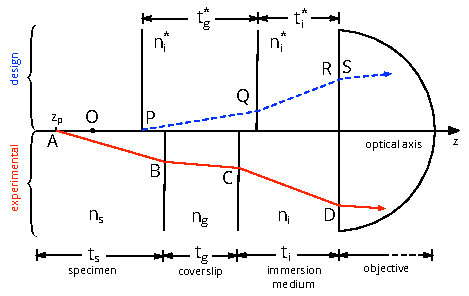
\includegraphics[width=0.7\textwidth]{gibson-lanni}
    %   \bcaption[Schematics for the Gibson-Lanni model]{The model is based on the differences in light propagation between the experimental (red) and design conditions (blue). The optical path length difference is calculated as follows: $OPD = [ABCD] - [PQRS]$. System properties are represented by vectors $\mathbf{n} = (n_i, n_i^*, n_g, n_g^*, n_s)$ and $\mathbf{t} = (t_i, t_i^*, t_g, t_g^*, t_s)$ for the refractive indices and path lengths respectively. Adapted from \cite{li_fast_2017}.}
    %   \label{fig:gibson-lanni}
    % \end{figure}

    \begin{figure}[htb]
      \centering
      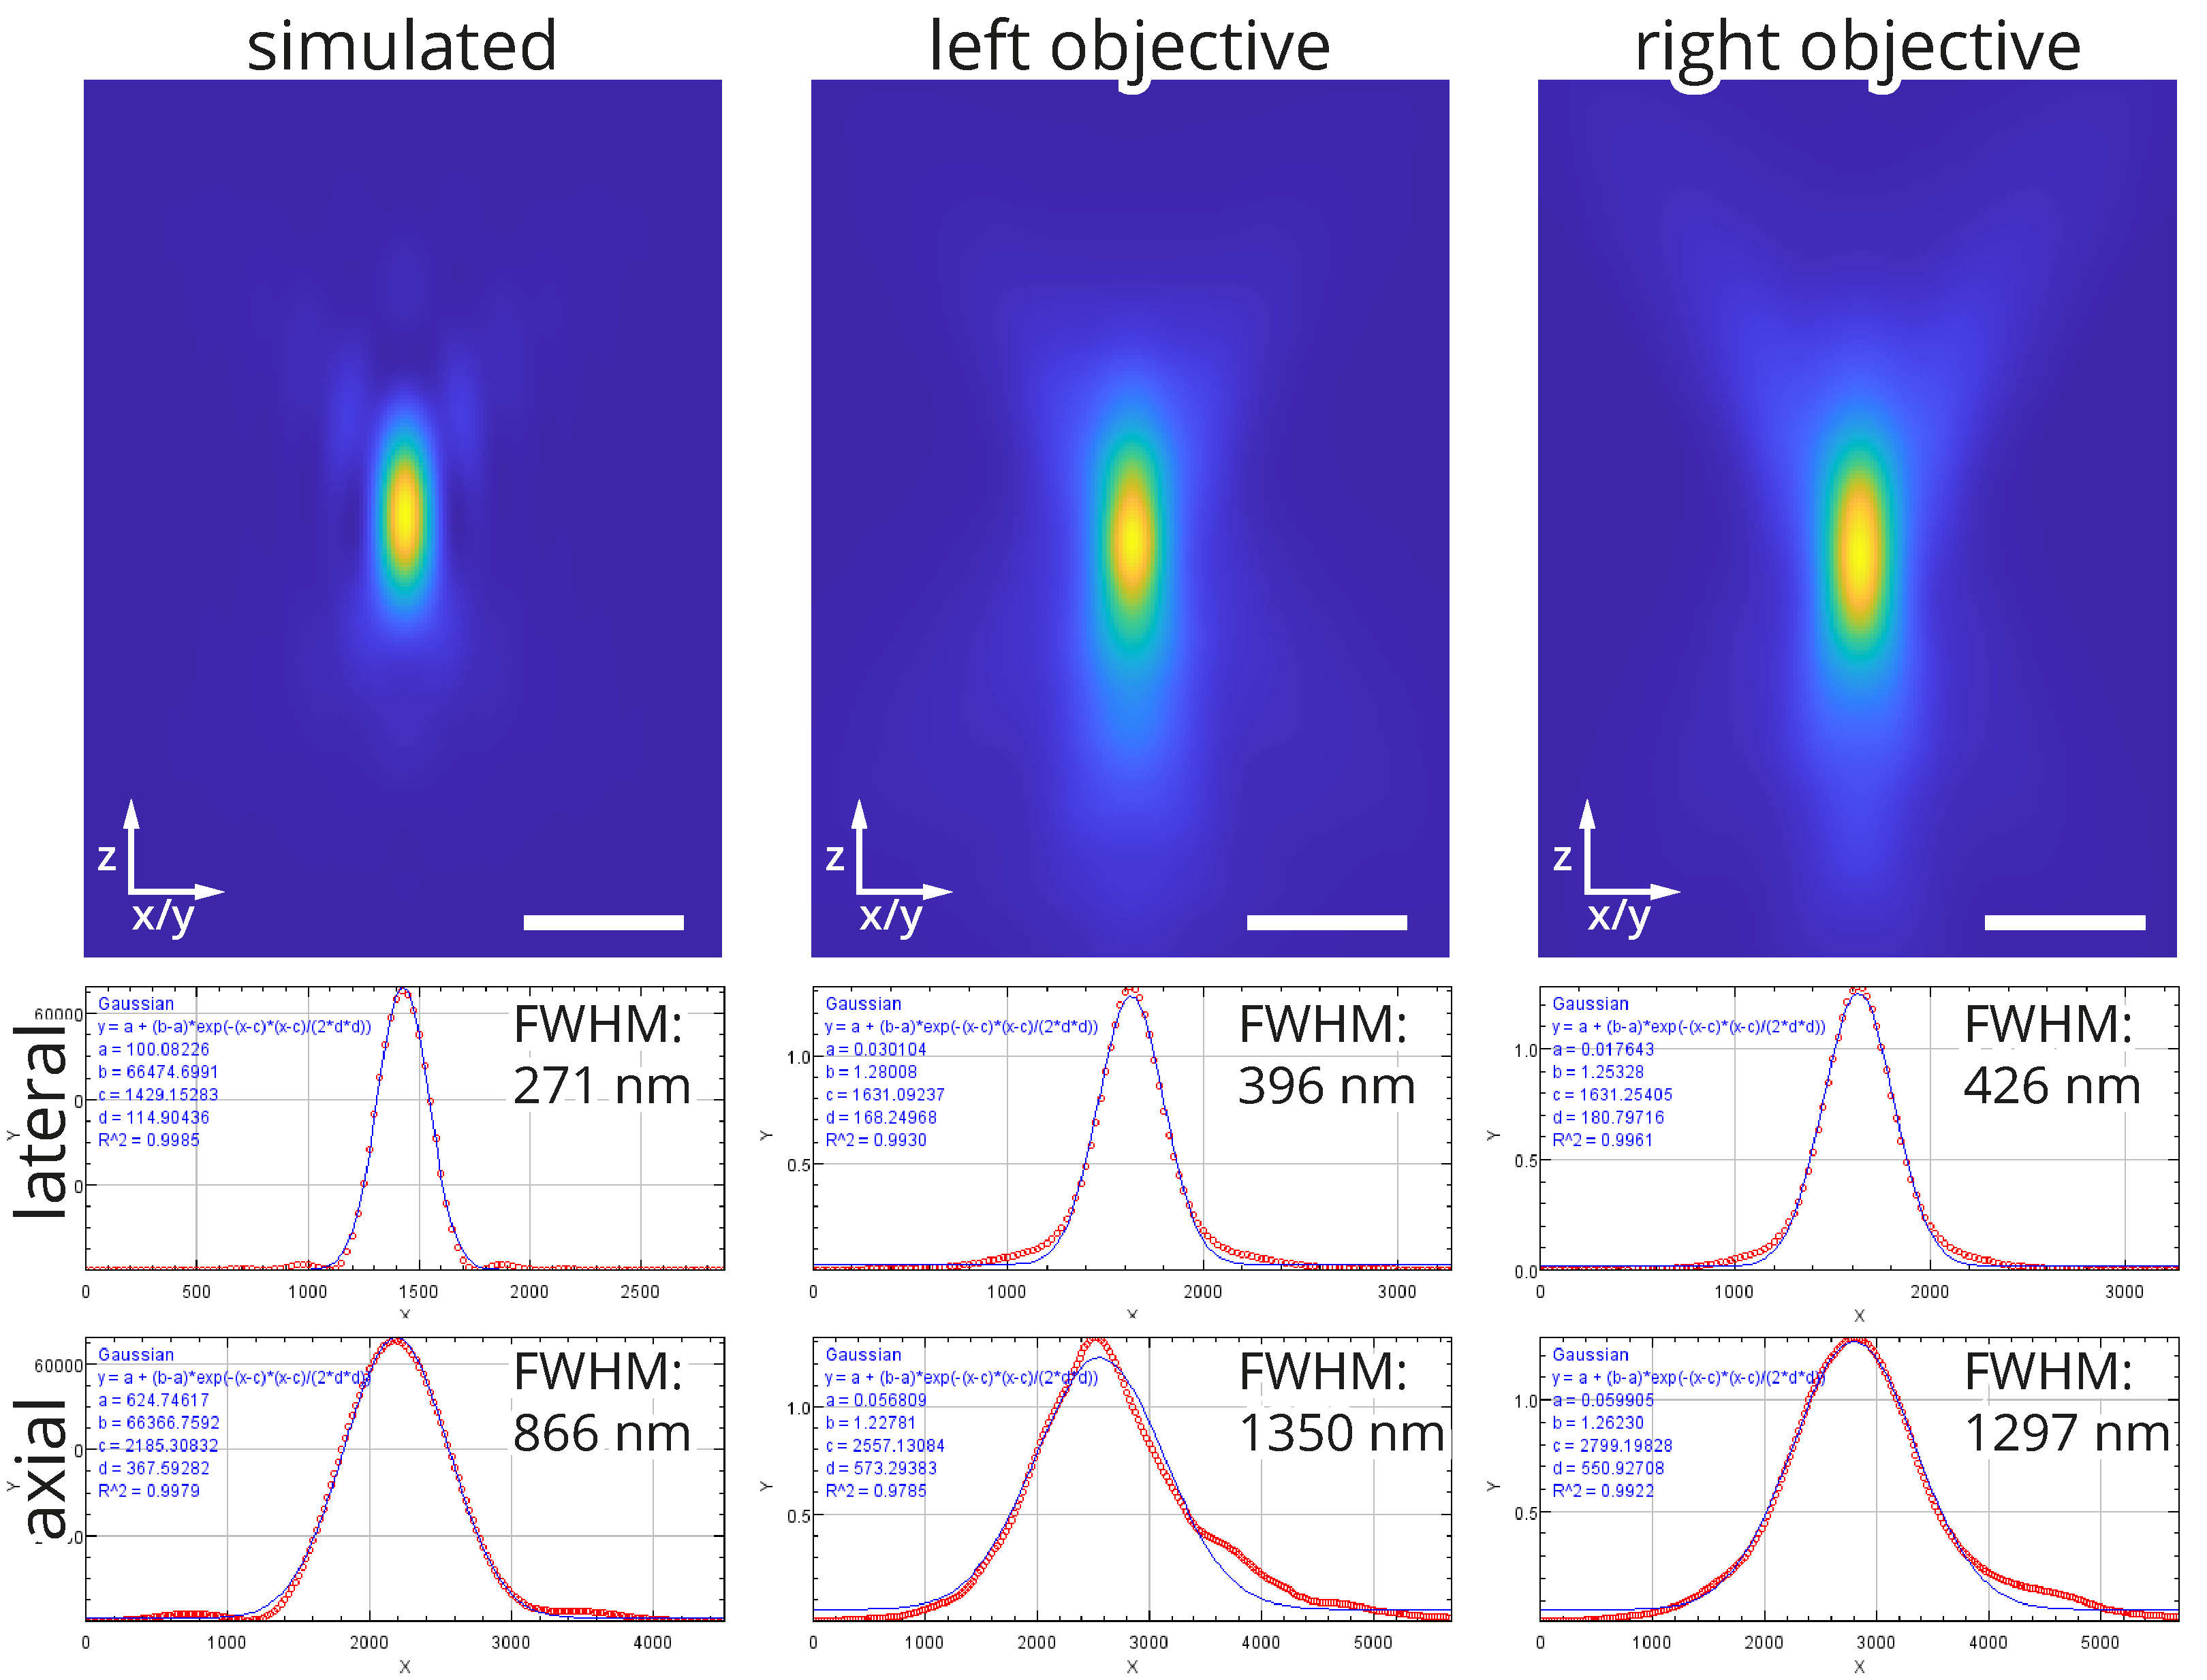
\includegraphics[width=\textwidth]{PSF}
      \bcaption[Simulated and measured PSF of Dual Mouse-SPIM]{Top row: axial sections of simulated and measured point spread functions. Middle row: lateral intensity profile and Gaussian fit. Bottom row: Axial intensity profile and Gaussian fit. Simulations were performed based on the Gibson-Lanni model. Immersion medium  and sample refractive index: 1.330, coverslip (FEP foil) refractive index: 1.344, coverslip distance: \SI{1900}{\micro m}, coverslip thickness: \SI{50}{\micro m}. Scale bar: \SI{500}{nm}.}
      \label{fig:measuredPSF}
    \end{figure}

  \subsection{Multi-view imaging of a mouse zygote}
    \begin{figure}[htb]
      \centering
      \includegraphics[width=.75\textwidth]{zygoteMontage}
      \bcaption[Multi-view recording of a mouse zygote]{Dual-view imaging was performed on a fixed mouse zygote. Microtubules wre stained with Alexa Fluor 488. Top row: view of Left objective. Bottom row: view of Right objective. (a) Raw image from left objective. (b) Rotated view of Right objective. (c) Multi-view deconvolution of stacks (a) and (b). (d) Rotated slice from left objective. (e) Raw image from right objective. (f) Multi-view deconvolution of stacks (d) and (e). Scale bar: \SI{50}{\micro m}.}
      \label{fig:zygoteMontage}
    \end{figure}


\section{Methods}

  \subsection{Bead imaging}
    For registration and resolution measurements we used TetraSpeck (ThermoFisher, T7279 and T7281) \SI{0.1}{\micro m} and \SI{0.5}{\micro m} diameter beads. The bead solutions were thoroughly vortexed and sonicated for \SI{5}{mins} before diluting them 1:100 in distilled water. GelRite (Sigma-Aldrich, G1910) gel was prepared in distilled water at 0.8\% concentration with 0.1\% $\mathrm{MgSO_4\cdot 7 H_2O}$ and kept at \SI{70}{\degree C} until use. 

  \subsection{Mouse zygote imaging}
    Fixed mouse zygotes labeled with Alexa-488 (microtubules) and Alexa-647 (kinetochores) were kindly provided by Judith Reichmann. Zygotes were transferred to the sample holder, and imaged in PBS. To allow for multi-view reconstruction, a fluorescent beads (TetraSpeck \SI{0.5}{\micro m} suspended in GelRite wre placed nex to the zygote in the sample holder. After imaging the zygote from both views, the beads were also recorded using the same stack definitions. After data acquisition, the multi-view datasets were registered and deconvolved in Fiji \cite{schindelin_fiji:_2012} using the Multiview Reconstruction Plugin \cite{preibisch_software_2010,preibisch_efficient_2014}. The deconvolution was based on a simulated PSF generated in Fiji using the PSF Generator plugin \cite{kirshner_3d_2011} using the Born-Wolf PSF model. $\mathrm{NA_{ex}}=0.1$, $\mathrm{NA_{em}}=1.1$, n=1.33, $\lambda_{ex} = \SI{488}{nm}$, $\lambda_{em} = \SI{510}{nm}$.

  \subsection{Drosophila embryo imaging}
    \textit{Drosophila melanogaster} embryos expressing fluorescent nuclear (H2A-mCherry) and centriole (ASL-YFP) markers were collected on an agar juice plate and dechorionated in 50\% bleach solution for \SI{1}{min}. After rinsing the bleach with deionized water, the embryos were placed in the sample holder under PBS solution. A small piece of gel containing fluorescent beads were also placed next to the samples to aid in multi-view registration.

  \subsection{Drosophila salivary gland imaging}
    Salivary glands from third instar larvae expressing fluorescent nuclear (H2A-mCherry) and centriole (ASL-YFP) markers were kindly provided by Ulla-Maj Fiuza. The salivary glands were imaged in PBS, together with a small piece of gel with fluorescent beads.
